% !TeX program = lualatex
\documentclass[fleqn]{NotesClass}

\strictpagecheck

%% Packages
\usepackage{csquotes}

\usepackage{siunitx}

% Tikz stuff
\usepackage{tikz}
%\tikzset{>=latex}
% £xternal
\usetikzlibrary{external}
\tikzexternalize[prefix=tikz-external/]
% Other libraries

\usepackage[compat=1.1.0]{tikz-feynman}

% References, should be last things loaded
\usepackage[pdfauthor={Willoughby Seago},pdftitle={Particle Physics},pdfkeywords={particle physics, Feynman diagrams, scattering, Dirac equation, QED, QCD, weak interactions},pdfsubject={Quantum Field Theory}]{hyperref}  % Should be loaded second last (cleveref last)
\colorlet{hyperrefcolor}{blue!60!black}
\hypersetup{colorlinks=true, linkcolor=hyperrefcolor, urlcolor=hyperrefcolor}
\usepackage[
capitalize,
nameinlink,
noabbrev
]{cleveref} % Should be loaded last

% My packages
\usepackage{NotesBoxes}
\usepackage{NotesMaths}

\setmathfont[range={\int, \oint}]{Latin Modern Math}

% Highlight colour
\definecolor{Burgandy}{HTML}{8F2D56}
\definecolor{Teal}{HTML}{218380}
\definecolor{Blue}{HTML}{73D2DE}
\definecolor{Pink}{HTML}{D81159}
\definecolor{Yello}{HTML}{FFBC42}

\colorlet{highlight}{Burgandy}

% Title page info
\title{Particle Physics}
\author{Willoughby Seago}
\date{}
% \subtitle{}
% \subsubtitle{}

% Commands

% Particles
\newcommand{\Pparticle}[1]{\symup{#1}}
\newcommand{\Pu}{\ensuremath{\Pparticle{u}}}
\newcommand{\Pd}{\ensuremath{\Pparticle{d}}}
\newcommand{\Ps}{\ensuremath{\Pparticle{s}}}
\newcommand{\Pc}{\ensuremath{\Pparticle{c}}}
\newcommand{\Pt}{\ensuremath{\Pparticle{t}}}
\newcommand{\Pb}{\ensuremath{\Pparticle{b}}}
\newcommand{\Pe}{\ensuremath{\Pparticle{e}^{-}}}
\newcommand{\Pmu}{\ensuremath{\Pparticle{\mu}^{-}}}
\newcommand{\Ptau}{\ensuremath{\Pparticle{\tau}^{-}}}
\newcommand{\Pnue}{\ensuremath{\Pparticle{\nu_{e}}}}
\newcommand{\Pnumu}{\ensuremath{\Pparticle{\nu_{\mu}}}}
\newcommand{\Pnutau}{\ensuremath{\Pparticle{\nu_{\tau}}}}
\newcommand{\PH}{\ensuremath{\Pparticle{H}}}
\newcommand{\PZ}{\ensuremath{\Pparticle{Z}}}
\newcommand{\PWpm}{\ensuremath{\Pparticle{W}^{\pm}}}
\newcommand{\PWp}{\ensuremath{\Pparticle{W}^{+}}}
\newcommand{\PWm}{\ensuremath{\Pparticle{W}^{-}}}
\newcommand{\Pphoton}{\ensuremath{\Pparticle{\gamma}}}
\newcommand{\Pg}{\ensuremath{\Pparticle{g}}}
\newcommand{\Pq}{\ensuremath{\Pparticle{q}}}
\newcommand{\Ppip}{\ensuremath{\Pparticle{\pi}^{+}}}
\newcommand{\Ppim}{\ensuremath{\Pparticle{\pi}^{-}}}



\newcommand{\APantiparticle}[1]{\overbar{#1}}
\newcommand{\APu}{\ensuremath{\APantiparticle{\Pparticle{u}}}}
\newcommand{\APd}{\ensuremath{\APantiparticle{\Pparticle{d}}}}
\newcommand{\APs}{\ensuremath{\APantiparticle{\Pparticle{s}}}}
\newcommand{\APc}{\ensuremath{\APantiparticle{\Pparticle{c}}}}
\newcommand{\APt}{\ensuremath{\APantiparticle{\Pparticle{t}}}}
\newcommand{\APb}{\ensuremath{\APantiparticle{\Pparticle{b}}}}
\newcommand{\APe}{\ensuremath{\Pparticle{e}^{+}}}
\newcommand{\APmu}{\ensuremath{\Pparticle{\mu}^{+}}}
\newcommand{\APtau}{\ensuremath{\Pparticle{\tau}^{+}}}
\newcommand{\APnue}{\ensuremath{\Pparticle{\APantiparticle{\nu}_{e}}}}
\newcommand{\APnumu}{\ensuremath{\Pparticle{\APantiparticle{\nu}_{\mu}}}}
\newcommand{\APnutau}{\ensuremath{\Pparticle{\APantiparticle{\nu}_{\tau}}}}
\newcommand{\APH}{\ensuremath{\Pparticle{H}}}
\newcommand{\APZ}{\ensuremath{\Pparticle{Z}}}
\newcommand{\APWpm}{\ensuremath{\Pparticle{W}^{\mp}}}
\newcommand{\APWp}{\ensuremath{\Pparticle{W}^{-}}}
\newcommand{\APWm}{\ensuremath{\Pparticle{W}^{+}}}
\newcommand{\APphoton}{\ensuremath{\Pparticle{\gamma}}}
\newcommand{\APg}{\ensuremath{\Pparticle{g}}}
\newcommand{\APq}{\ensuremath{\APantiparticle{\Pparticle{q}}}}

% Maths
\newcommand{\strongCoupling}{g_{\symrm{s}}}
\newcommand{\wCoupling}{g_{\symrm{W}}}
\newcommand{\zCoupling}{g_{\symrm{Z}}}

\includeonly{}

\begin{document}
    \frontmatter
    \titlepage
    \innertitlepage{}
    \tableofcontents
    \listoffigures
    \mainmatter
    
    \chapter{Introduction}
    \section{The Standard Model}
    The \defineindex{standard model of particle physics}, or the standard model for short, is our best model of the fundamental constituents of matter and fundamental forces.
    The standard model actually refers to a collection of quantum field theories (QFT)\glossary[acronym]{QFT}{Quantum Field Theory} describing these forces as due to particle exchanges.
    The standard model is theoretically self consistent, all of the maths checks out.
    It can be used to make predictions, which can then be checked against measurements.
    So far all such tests have validated the standard model.
    As a model the standard model does not predict everything, instead there are about 20 parameters that have to be measured separately, including the masses of various particles, the coupling strengths of various fields, and mixing parameters.
    
    The standard model cannot explain everything, a nonexhaustive list of unexplained phenomena by the standard model is as follows:
    \begin{itemize}
        \item general relativity/accelerating expansion of the universe;
        \item dark energy/dark matter;
        \item neutrino masses;
        \item matter/antimatter imbalance;
        \item why the parameters have the values they do.
    \end{itemize}
    
    \section{Fundamental Particles}
    \epigraph{A particle with no charge. What's the point in that?}{Victoria Marting}
    \define{Spin}\index{spin} is a property that every particle has, it's a quantum number, just a label, like charge or mass, but without such a simple interpretation.
    There are two spin operators, the total spin operator, \(\operator{S}^2\), and the component of spin in the \(z\)-direction, \(\operator{S}_z\).
    If \(\ket{\psi}\) is a spin eigenstate then the action of these operators on \(\ket{\psi}\) is
    \begin{equation}
        \operator{S}^2 \ket{\psi} = s(s + 1)\ket{\psi}, \qand \operator{S}_z \ket{\psi} = m_s \hbar \ket{\psi}.
    \end{equation}
    Here \(s\) takes on a nonnegative half integer value, \(s = 0, \pm 1/2, \pm 1, \pm 3/2, \dotsc\).
    The value of \(m_s\) is then constrained to lie between \(-s\) and \(s\) increasing in integer steps, so \(m_s = -s, 1 - s, \dotsc, 0, \dotsc, s - 1, s\).
    
    The fundamental particles in the standard model have spin \(s = 0, 1/2, 1\).
    Specifically, the Higgs boson has spin 0, the quarks and leptons have spin \(1/2\), and the force carriers have spin 1.
    When a particle has spin \(1/2\) there are two possible values of \(m_s\), \(\pm 1/2\), which we call spin up (\(+1/2\)) and spin down (\(-1/2\)).
    When a particle has spin \(1\) there are three possible values of \(m_s\), \(0\) and \(\pm 1\), which we refer to as polarisations.
    A photon can only have \(m_s = \pm 1\), which is where this terminology comes from.
    
    We broadly split all particles into two types, \define{fermions}\index{fermion}, with half integer spin, and \define{bosons}\index{boson}, with integer spin.
    The fermions in the standard model further split into \define{quarks}\index{quark} and \define{leptons}\index{lepton}.
    
    There are 6 quarks, which split into two types up-type, \define{up}\index{up quark}, \define{charm}\index{charm quark}, and \define{top quarks}\index{top quark}, or \Pu\index{u@\Pu|see{up quark}}, \Pc\index{c@\Pc|see{charm quark}}, and \Pt\index{t@\Pt|see{top quark}}, and down-type quarks, the \define{down}\index{down quark}, \define{strange}\index{strange quark}, and \define{bottom quarks}\index{bottom quark}, or \Pd\index{d@\Pd|see{down quark}}, \Ps\index{s@\Ps|see{strange quark}}, and \Pb\index{b@\Pb|see{bottom quark}}.
    Up-type quarks have charge \(+2/3\) in units of electron charge, and bottom-type quarks have charge \(-1/3\).
    All types of quarks also have \enquote{colour charge}, relating to the strong force, and \enquote{weak isospin}, relating to the weak force, we'll see this in more detail later in the course.
    Each type (up/down) consists of three generations of quarks, and as we go down the generations, from \Pu{}, to \Pc, to \Pt, they get more massive.
    
    Similarly the leptons are split into two, first we have \define{electrons}\index{electron}, \Pe\index{e-@\Pu|see{electron}}, \define{muons}\index{muon}, \Pmu\index{\Pmu|see{muon}}, and \define{tau}\index{tau lepton} particles, \Ptau\index{\Ptau|see{tau lepton}}, these all have a charge of \(-1\).
    Then, there are the three \define{neutrinos}\index{neutrino}, the \define{electron}\index{electron neutrino}, \define{muon}\index{muon neutrino}, and \define{tau neutrinos}\index{tau neutrino}, \Pnue\index{\Pnue|see{electron neutrino}}, \Pnumu\index{\Pnumu|see{muon neutrino}}, and \Pnutau\index{\Pnutau|see{tau neutrino}}, these are all electrically neutral.
    All leptons have zero colour charge, but they do have weak isospin.
    
    We split the bosons into two parts, the spin zero bosons, or \define{scalar bosons}\index{scalar boson}, which is just the \defineindex{Higgs boson}, \PH\index{H@\PH|see{Higgs boson}}.
    Then there are the force carrying bosons, also known as \define{gauge bosons}\index{gauge bosons} or \define{vector bosons}\index{vector boson}, which have spin 1.
    These consist of the \defineindex{photon}, \Pphoton\index{\Pphoton|see{photon}}, gluons, \Pg\index{g@\Pg|see{gluon}}, \defineindex{\PZ{} boson}, and \defineindex{\PWpm{}-bosons}.
    The photon is the force carrier in electromagnetism and quantum electrodynamics (QED)\glossary[acronym]{QED}{Quantum Electrodynamics}.
    The gluons are the force carriers in quantum chromodynamics (QCD)\glossary[acronym]{QCD}{Quantum Chromodynamics}.
    The \PZ-boson gives neutral currents in weak interactions and \PWpm-bosons give charged currents.
    Finally, there is the hypothetical graviton, which if it exists will be a spin 2 boson, or a \defineindex{tensor boson}.
    Note that these names, scalar, vector, and gauge, come from what type of object the fields describing the particle are, so the photon is described by the electromagnetic field, \(A^\mu\), whereas the graviton is described by the energy-momentum tensor, \(T^{\mu\nu}\).
    
    \begin{figure}
        \tikzsetnextfilename{standard-model}
        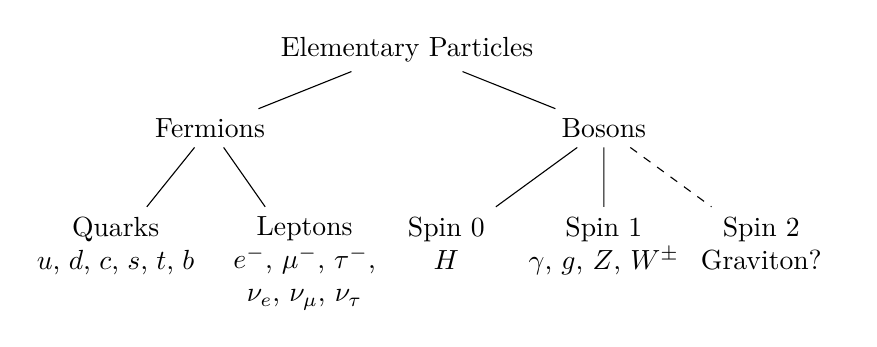
\begin{tikzpicture}[
            level 1/.style = {sibling distance = 5cm},
            level 2/.style = {sibling distance = 2cm, anchor=north}
            ]
            \node {Elementary Particles}
            child {node {Fermions}
                child {node [xshift=-0.2cm] {\parbox{2cm}{\centering Quarks\\ \Pu, \Pd, \Pc, \Ps, \Pt, \Pb}}}
                child {node [xshift=0.2cm] {\parbox{2cm}{\centering Leptons\\ \Pe, \Pmu, \Ptau, \Pnue, \Pnumu, \Pnutau}}}
            }
            child {node {Bosons}
                child {node {\parbox{2cm}{\centering Spin 0\\ \PH}}}
                child {node {\parbox{2cm}{\centering Spin 1\\ \Pphoton, \Pg, \PZ, \PWpm}}}
                child [dashed] {node {\parbox{2cm}{\centering Spin 2\\ Graviton?}}}
            };
        \end{tikzpicture}
        \caption{All of the particles in the standard model. The graviton is hypothesised but has not been observed.}
    \end{figure}
    
    \subsection{Antiparticles}
    Every particle has a corresponding \defineindex{antiparticle}, although some particles are there own antiparticles, such as the photon, Higgs boson, and \PZ{} boson.
    The \PWp{} and \PWm{} are mutually each others antiparticles, and the antiparticle of a gluon is another gluon.
    The antiparticles are defined by being identical, but with opposite charges.
    By charges here we mean electric charge, colour charge, and weak isospin, which are the charges telling us how strongly the particle couples to the electromagnetic field, strong force, and weak force respectively.
    
    The naming convention is to just stick the prefix \enquote{anti} in front of the particle's name.
    The one exception to the naming convention is the electron, whose antiparticle is the \defineindex{positron}.
    Most antiparticles are denoted as the same symbol with a bar, so \APu{} is an antiup quark.
    If the symbol usually has a sign, such as \Pe, or \PWp, then the antiparticle is denoted with the opposite sign, so \APe\index{e+@\APe|see{positron}}, or \PWm.
    
    \section{Composite Particles}
    As well as the fundamental particles, of which there are 18 particles, there are \emph{a lot} of \define{composite particles}\index{composite particle}, particles formed by combining quarks and/or antiquarks into a bound state.
    Note that there aren't composite leptons because the strong force is required to form bound states.
    
    We call a composite particle formed from quarks a \defineindex{hadron}.
    The hadrons split two types, first \define{baryons}\index{baryon}, which are formed of three quarks\footnote{here \Pq{} denotes an arbitrary quark, in particular there is no requirement that all three quarks in a baryon are the same, even if we call all three \Pq.}, \Pq\Pq\Pq, and \define{antibaryons}\index{antibaryon}, which are formed of three antiquarks, \APq\APq\APq.
    The other class is \define{mesons}\index{meson}, which are quark-antiquark pairs, \Pq\APq.
    
    The antiparticle of a composite particle has its quarks replaced with the equivalent antiquarks, and antiquarks replaced with the equivalent quarks.
    For example, the \defineindex{negative pion}, \Ppim\index{\Ppim|see{negative pion}}, is a meson with quark content \Pd\APu, and its antiparticle is the \defineindex{positive pion}, \Ppip\index{\Ppip|see{positive pion}}, another meson with quark content \Pu\APd.
    
    As well as the hadrons and mesons there have been other composite particles observed recently, although these aren't on the course as they aren't well understood yet.
    We've seen \defineindex{tetraquarks}, formed from two quarks and two antiquarks, \Pq\Pq\APq\APq, and pentaquarks, formed from four quarks and an antiquark, \Pq\Pq\Pq\Pq\APq.
    It is possible that these states aren't really new particles, but instead are \enquote{molecules} of either pairs of mesons in the tetraquark case or a hadron and a meson in the pentaquark case.
    The difference being that in the \enquote{molecules} not all quarks would be equally bound to each other, whereas if they truly are composite particles there will be no difference in how bound any pair is, apart from, for example, differences due to differing electric charges.
    
    \chapter{Feynman Diagrams}
    \define{Feynman diagrams}\index{Feynman diagram} are a way of depicting interactions between particles.
    They also correspond to the amplitude for that interaction occurring in that way.
    Each piece of the diagram can be converted into a term in some expression for the amplitude.
    More abstractly we can view Feynman diagrams as terms in a series expansion of some amplitude.
    
    When reading Feynman diagrams in this course we follow the convention that time increases to the right.
    
    \section{Currents}
    The most basic part of a Feynman diagram is a \enquote{current}.
    This is a line representing the movement of a particle through spacetime.
    The phrase current comes from electrons, where an electron moving through space is interpreted as a current.
    
    The way we depict a current depends on the type of particle.
    Fermions are depicted as a straight line with an arrow, so a fermion current looks like
    \begin{equation}
        \tikzsetnextfilename{fd-fermion-current}
        \feynmandiagram [horizontal=i to o] {
            i -- [fermion] o
        };
        .
    \end{equation}
    Antifermions are then depicted as fermions travelling back in time, so an antifermion current looks like
    \begin{equation}
        \tikzsetnextfilename{fd-antifermion-current}
        \feynmandiagram [horizontal=i to o] {
            i -- [anti fermion] o
        };
        .
    \end{equation}
    Spin 1 bosons, apart from gluons, so photons, \PZ{} bosons, and \PWpm{} bosons, are depicted with a wavy line:
    \begin{equation}
        \tikzsetnextfilename{fd-boson-current}
        \feynmandiagram [horizontal=i to o] {
            i -- [boson] o
        };
        .
    \end{equation}
    Gluons are depicted with a curly line,
    \begin{equation}
        \tikzsetnextfilename{fd-gluon-current}
        \feynmandiagram [horizontal=i to o] {
            i -- [gluon] o
        };
        .
    \end{equation}
    The Higgs boson is depicted with a dashed line,
    \begin{equation}
        \tikzsetnextfilename{fd-higgs-current}
        \feynmandiagram [horizontal=i to o] {
            i -- [scalar] o
        };
        .
    \end{equation}
    
    It's fine not to draw an arrow for bosons as either the particle is its own antiparticle, in which case the direction does not matter, or in the case of the \PWpm{} bosons or gluons the antiparticle is of the same type, so changing direction corresponds to changing the charge (electric charge for \PWpm, and colour charge for gluons).
    
    \section{Vertex}
    The building block of any Feynman diagram is the \defineindex{vertex}, this is where currents come together.
    The exact rules for which currents can form a vertex depends on the theory in question.
    A vertex is not, by itself, a valid process.
    Instead, a diagram is a combination of vertices, connected in such a way that all conservation laws are obeyed.
    
    For now we focus on vertices involving a fermion.
    These will always have exactly two fermion currents and a boson current, so for example,
    \begin{equation}
        \tikzsetnextfilename{fd-vertex}
        \feynmandiagram [horizontal=i to v, inline=(i)] {
            i -- [fermion] v,
            v -- [boson] o1,
            v -- [fermion] o2
        };
        .
    \end{equation}
    
    If we want to specify particular particles we can do so by labelling the lines:
    \begin{equation}
        \tikzsetnextfilename{fd-vertex-muon-photon}
        \feynmandiagram [horizontal=i to v, inline=(i)] {
            i [particle=\Pmu] -- [fermion] v,
            v -- [boson] o1 [particle=\Pphoton],
            v -- [fermion] o2 [particle=\Pmu]
        };
        \qqand
        \tikzsetnextfilename{fd-vertex-strange-gluon}
        \feynmandiagram [horizontal=i to v, inline=(i)] {
            i [particle=\Ps] -- [fermion] v,
            v -- [gluon] o1 [particle=\Pg],
            v -- [fermion] o2 [particle=\Ps]
        };
        .
    \end{equation}
    These represent the processes \(\Pmu \to \Pmu\Pphoton\) and \(\Ps \to \Ps\Pg\).
    
    At every vertex there are conservation laws we have to apply.
    Again, the details depend on exactly what the fermions and bosons are.
    We must always conserve energy, momentum, and charge.
    There are also other quantities that must be conserved, such as muon lepton number, which is the number of muons and muon neutrinos minus the number of antimuons and antimuon neutrinos.
    We must also conserve the quark number, which is the number of quarks minus the number of antiquarks.
    
    Energy and momentum conservation can be combined into conservation of four-momentum, where
    \begin{equation}
        p^\mu = (E/c, \vv{p})
    \end{equation}
    is the four-momentum of a particle with energy \(E\) and momentum \(\vv{p}\).
    
    Given a valid vertex if we rotate it we will get another valid vertex.
    For example, rotating the \(\Ps \to \Ps\Pg\) vertex above we get the vertices
    \begin{equation}
        \tikzsetnextfilename{fd-vertex-strange-gluon-rotated-1}
        \feynmandiagram [horizontal=i to v, inline=(v)] {
            i [particle=\Pg] -- [gluon] v,
            v -- [fermion] o1 [particle=\Ps],
            v -- [anti fermion] o2 [particle=\APs]
        };
        \qqand
        \tikzsetnextfilename{fd-vertex-strange-gluon-rotated-2}
        \feynmandiagram [horizontal=v to o, inline=(v)] {
            i1 [particle=\Ps] -- [fermion] v,
            i2 [particle=\APs] -- [anti fermion] v,
            v -- [gluon] o [particle=\Pg] 
        };
        .
    \end{equation}
    The only thing that changes here is the interpretation, these processes now represent \(\Pg \to \Ps\APs\) and \(\Ps\APs \to \Pg\).
    
    \subsection{Forces}
    \subsubsection{Electromagnetic Vertex}
    An electromagnetic vertex has a photon and any charged fermion.
    If the fermion has charge \(Q\) then the coupling constant, which we'll see later relates to how strong the interaction is, is \(Q\).
    There will be no fermion flavour change.
    \begin{equation}
        \tikzsetnextfilename{fd-vertex-electromagnetic-vertex}
        \begin{tikzpicture}[baseline=(i)]
            \begin{feynman}[horizontal=i to v, inline=(i)]
                \diagram{
                    i -- [fermion] v,
                    v -- [boson] o1 [particle=\Pphoton],
                    v -- [fermion] o2,
                };
                \node [right] at (v) {\(Q\)};
            \end{feynman}
        \end{tikzpicture}
    \end{equation}
    
    \subsubsection{Strong Vertex}
    A strong vertex has a gluon and a quark.
    The coupling constant is \(\strongCoupling\).
    There will be no quark flavour change.
    \begin{equation}
        \tikzsetnextfilename{fd-vertex-strong-vertex}
        \begin{tikzpicture}[baseline=(i)]
            \begin{feynman}[horizontal=i to v, inline=(i)]
                \diagram{
                    i [particle=\Pq] -- [fermion] v,
                    v -- [gluon] o1 [particle=\Pg],
                    v -- [fermion] o2 [particle=\Pq],
                };
                \node [right, xshift=0.1cm] at (v) {\(\strongCoupling\)};
            \end{feynman}
        \end{tikzpicture}
    \end{equation}
    
    \subsubsection{Neutral Current Weak Vertex}
    A neutral current weak vertex has a \PZ{} boson and any fermion.
    The coupling constant is \(\zCoupling\).
    There will be no fermion flavour change.
    \begin{equation}
        \tikzsetnextfilename{fd-vertex-weak-neutral-vertex}
        \begin{tikzpicture}[baseline=(i)]
            \begin{feynman}[horizontal=i to v, inline=(i)]
                \diagram{
                    i -- [fermion] v,
                    v -- [boson] o1 [particle=\PZ],
                    v -- [fermion] o2,
                };
                \node [right] at (v) {\(\zCoupling\)};
            \end{feynman}
        \end{tikzpicture}
    \end{equation}
    
    \subsubsection{Charged Current Weak Vertex}
    A charged current weak vertex has a \PWpm{} boson and any fermion.
    The coupling constant is \(\wCoupling\).
    There will always be a fermion flavour change since it is required for charge conservation.
    \begin{equation}
        \tikzsetnextfilename{fd-vertex-weak-charged-vertex}
        \begin{tikzpicture}[baseline=(i)]
            \begin{feynman}[horizontal=i to v, inline=(i)]
                \diagram{
                    i [particle=\(\symrm{f}\)] -- [fermion] v,
                    v -- [boson] o1 [particle=\PWpm],
                    v -- [fermion] o2 [particle=\(\symrm{f}'\)],
                };
                \node [right] at (v) {\(Q\)};
            \end{feynman}
        \end{tikzpicture}
    \end{equation}
    
     %   Appdendix
    \appendixpage
    \begin{appendices}
        \chapter{List of Particles}
        \section{Fundamental Particles}
        \subsection{Fermions}
        \subsubsection{Leptons}
        \begin{center}
            \begin{tabular}{lcrSl}\toprule
                Particle & Symbol & Charge & Mass & \\ \hline
                Electron & \Pe & \(-1\) & 511.0 & \si{\kilo\electronvolt} \\
                Muon & \Pmu & \(-1\) & 105.6 & \si{\mega\electronvolt} \\
                Muon & \Ptau & \(-1\) & 1776.9 & \si{\mega\electronvolt} \\
                Electron Neutrino & \Pnue & \(0\) & < 0.120 & \si{\electronvolt} \\
                Muon Neutrino & \Pnumu & \(0\) & < 0.120 & \si{\electronvolt} \\
                Tau Neutrino & \Pnutau & \(0\) & < 0.120 & \si{\electronvolt} \\
                \bottomrule
            \end{tabular}
        \end{center}
    
        \subsubsection{Quarks}
        \begin{center}
            \begin{tabular}{lcrSl}\toprule
                Particle & Symbol & Charge & Mass & \\ \hline
                Up Quark & \Pu & \(+2/3\) & 2.3 & \si{\mega\electronvolt} \\
                Down Quark & \Pd & \(-1/3\) & 4.8 & \si{\mega\electronvolt} \\
                Charm Quark & \Pc & \(+2/3\) & 1.275 & \si{\giga\electronvolt} \\
                Strange Quark & \Ps & \(-1/3\) & 95 & \si{\mega\electronvolt} \\
                Top Quark & \Pt & \(+2/3\) & 173.2 & \si{\giga\electronvolt} \\
                Bottom Quark & \Pb & \(-1/3\) & 4.18 & \si{\giga\electronvolt} \\
                \bottomrule
            \end{tabular}
        \end{center}
        
        \subsubsection{Vector Bosons}
        \begin{center}
            \begin{tabular}{lcrSl}\toprule
                Particle & Symbol & Charge & Mass & \\ \hline
                Photon & \Pphoton & \(0\) & 0 & \\
                Gluon & \Pg & \(0\) & 4.8 & \\
                \PZ{} boson & \PZ & \(0\) & 91.19 & \si{\giga\electronvolt} \\
                \PWpm{} boson & \PWpm & \(\pm 1\) & 80.38 & \si{\giga\electronvolt} \\
                \bottomrule
            \end{tabular}
        \end{center}
        Note that recent measurements place the mass of the \PWpm{} boson at the slightly higher value of \qty{80.43}{\giga\electronvolt}.
        
        \subsubsection{Scalar Bosons}
        \begin{center}
            \begin{tabular}{lcrSl}\toprule
                Particle & Symbol & Charge & Mass & \\ \hline
                Higgs Boson & \PH & \(0\) & 125.25 & \si{\giga\electronvolt} \\
                \bottomrule
            \end{tabular}
        \end{center}
    \end{appendices}
    
    \backmatter
    \renewcommand{\glossaryname}{Acronyms}
    \printglossary[acronym]
    \printindex
\end{document}